
%version 2: \usepackage{hyperref}


%%%%%%%%%%%%%%%%%%%%%%%%%%%%%%%%%%%%%%%%%%%%%%%%%%%%%%%%%%%%%%%%%%%%%%%%
%Para las ecuaciones siempre es Ec.(n).
%Para las figuras siempre es Fig.n, incluso en el caption de la figura. Tambien las Tablas
%Para las referencias es [n]
%%%%%%%%%%%%%%%%%%%%%%%%%%%%%%%%%%%%%%%%%%%%%%%%%%%%%%%%%%%%%%%%%%%%%%%%

\documentclass[
reprint,
%notitlepage,
%superscriptaddress,
%groupedaddress,
%unsortedaddress,
%runinaddress,
%frontmatterverbose, 
%preprint,
%showpacs,preprintnumbers,
%nofootinbib,
%nobibnotes,
%bibnotes,
%11 pt,
amsmath,
amssymb,
aps,
pra,
%prb,
%rmp,
%tightenlines %esto hizo el milagro de sacar los espacios en blancos estocásticos (?)
%prstab,
%prstper,
%floatfix,\textbf{}
]{revtex4-1} %Instalar primero para usarlo. Paquete malo.

%\documentclass[onecolumn, aps, amsmath,amssymb ]{article}
\usepackage{lipsum}  
\usepackage{graphicx}% Include figure files
\usepackage{subfig}
\usepackage{braket}
\usepackage{comment} %comment large chunks of text
\usepackage{dcolumn}% Align table columns on decimal point
\usepackage{bm}% bold math
%\usepackage{hyperref}% add hypertext capabilities
\usepackage[mathlines]{lineno}% Enable numbering of text and display math
%\linenumbers\relax % Commence numbering lines
\usepackage{mathtools} %% Para el supraíndice

\usepackage[nice]{nicefrac}

%%%%%%%El Señor Español%%%%%%%%%%%%%%%%%%%%%%%%%%%
\usepackage[utf8]{inputenc} %acento
\usepackage[
spanish, %El lenguaje.
es-tabla, %La tabla y no cuadro.
activeacute, %El acento.
es-nodecimaldot %Punto y no coma con separador de números
]{babel}
\usepackage{microtype} %para hacerlo más bonito :33 como vos (?) 
%%%%%%%%%%%%%%%%%%%%%%%%%%%%%%%%%%%%%%%%%%%%%%%%%%%
%%%%%%%%% Para que las imágenes se queden dónde las quiero (?
\usepackage{float}
%%%%%%%%%%

\usepackage{hyperref} % Para usar \url

%%%%%%%%Cambia a Fig de Figure%%%%%%%%%%
\makeatletter
\renewcommand{\fnum@figure}{Fig. \thefigure} 
\makeatother
%%%%%%%%%%%%%%%%%%%%%%%%%%%%%%%%%%%%%%%%
\raggedbottom

\usepackage{scalerel}
\usepackage{physics}

\begin{document}
%%%%%%%%%%%%%%%%%%%%%%%%%%%%%%%%%%Título%%%%%%%%%%%%%%%%%%%%%%%%%%%%%%%%%%%%%%
%%%%%%%%%%%%%%%%%%%%%%%%%%%%%%%%%%%%%%%%%%%%%%%%%%%%%%%%%%%%%%%%%%%%%%%%%%%%%%

\title{Main Array vs. All Triggers}
\author{Evelyn~G.~Coronel}

\affiliation{
Tesis de Maestría en Ciencias Físicas\\ Instituto Balseiro\\}

\date[]{\lowercase{\today}} %%lw para lw, [] sin date

\maketitle

\subsection*{Nota sobre nomenclatura}
Cuando digo `Main Array' me estoy refiriendo al Main Array con el disparo estándar.

MA: Main Array.

AT: All Triggers.

Cuando digo rango 20xx - 20yy, quiero decir desde el 1 de enero del 20xx 00:00:00 GMT hasta el 1 de enero del 20yy 00:00:00 GMT
\section*{Main Array vs. All Triggers}

Para comparar las reconstrucciones de eventos de los disparos, tomé los eventos del MA y de AT desde el 2014 hasta fines del 2019. Comparé los valores de los \verb|AugerID| y yuxtapuse los valores S1000, S38 y energía según están los archivos del Herald.

Otro detalle es que solo estoy comparando los eventos filtrados según 6T5 con $\theta<60^o$, además de los filtros que recomiendo el Herald.

La figura \ref{fig:s1000versus} tiene una comparación de los valores de la señal de S1000 sin corregir por el clima para eventos coincidentes.  La línea negra representa la recta x, donde los punto debería caer si la señal fuera la misma para ambos disparos.

\begin{figure}[H]
    \begin{small}
        \begin{center}
            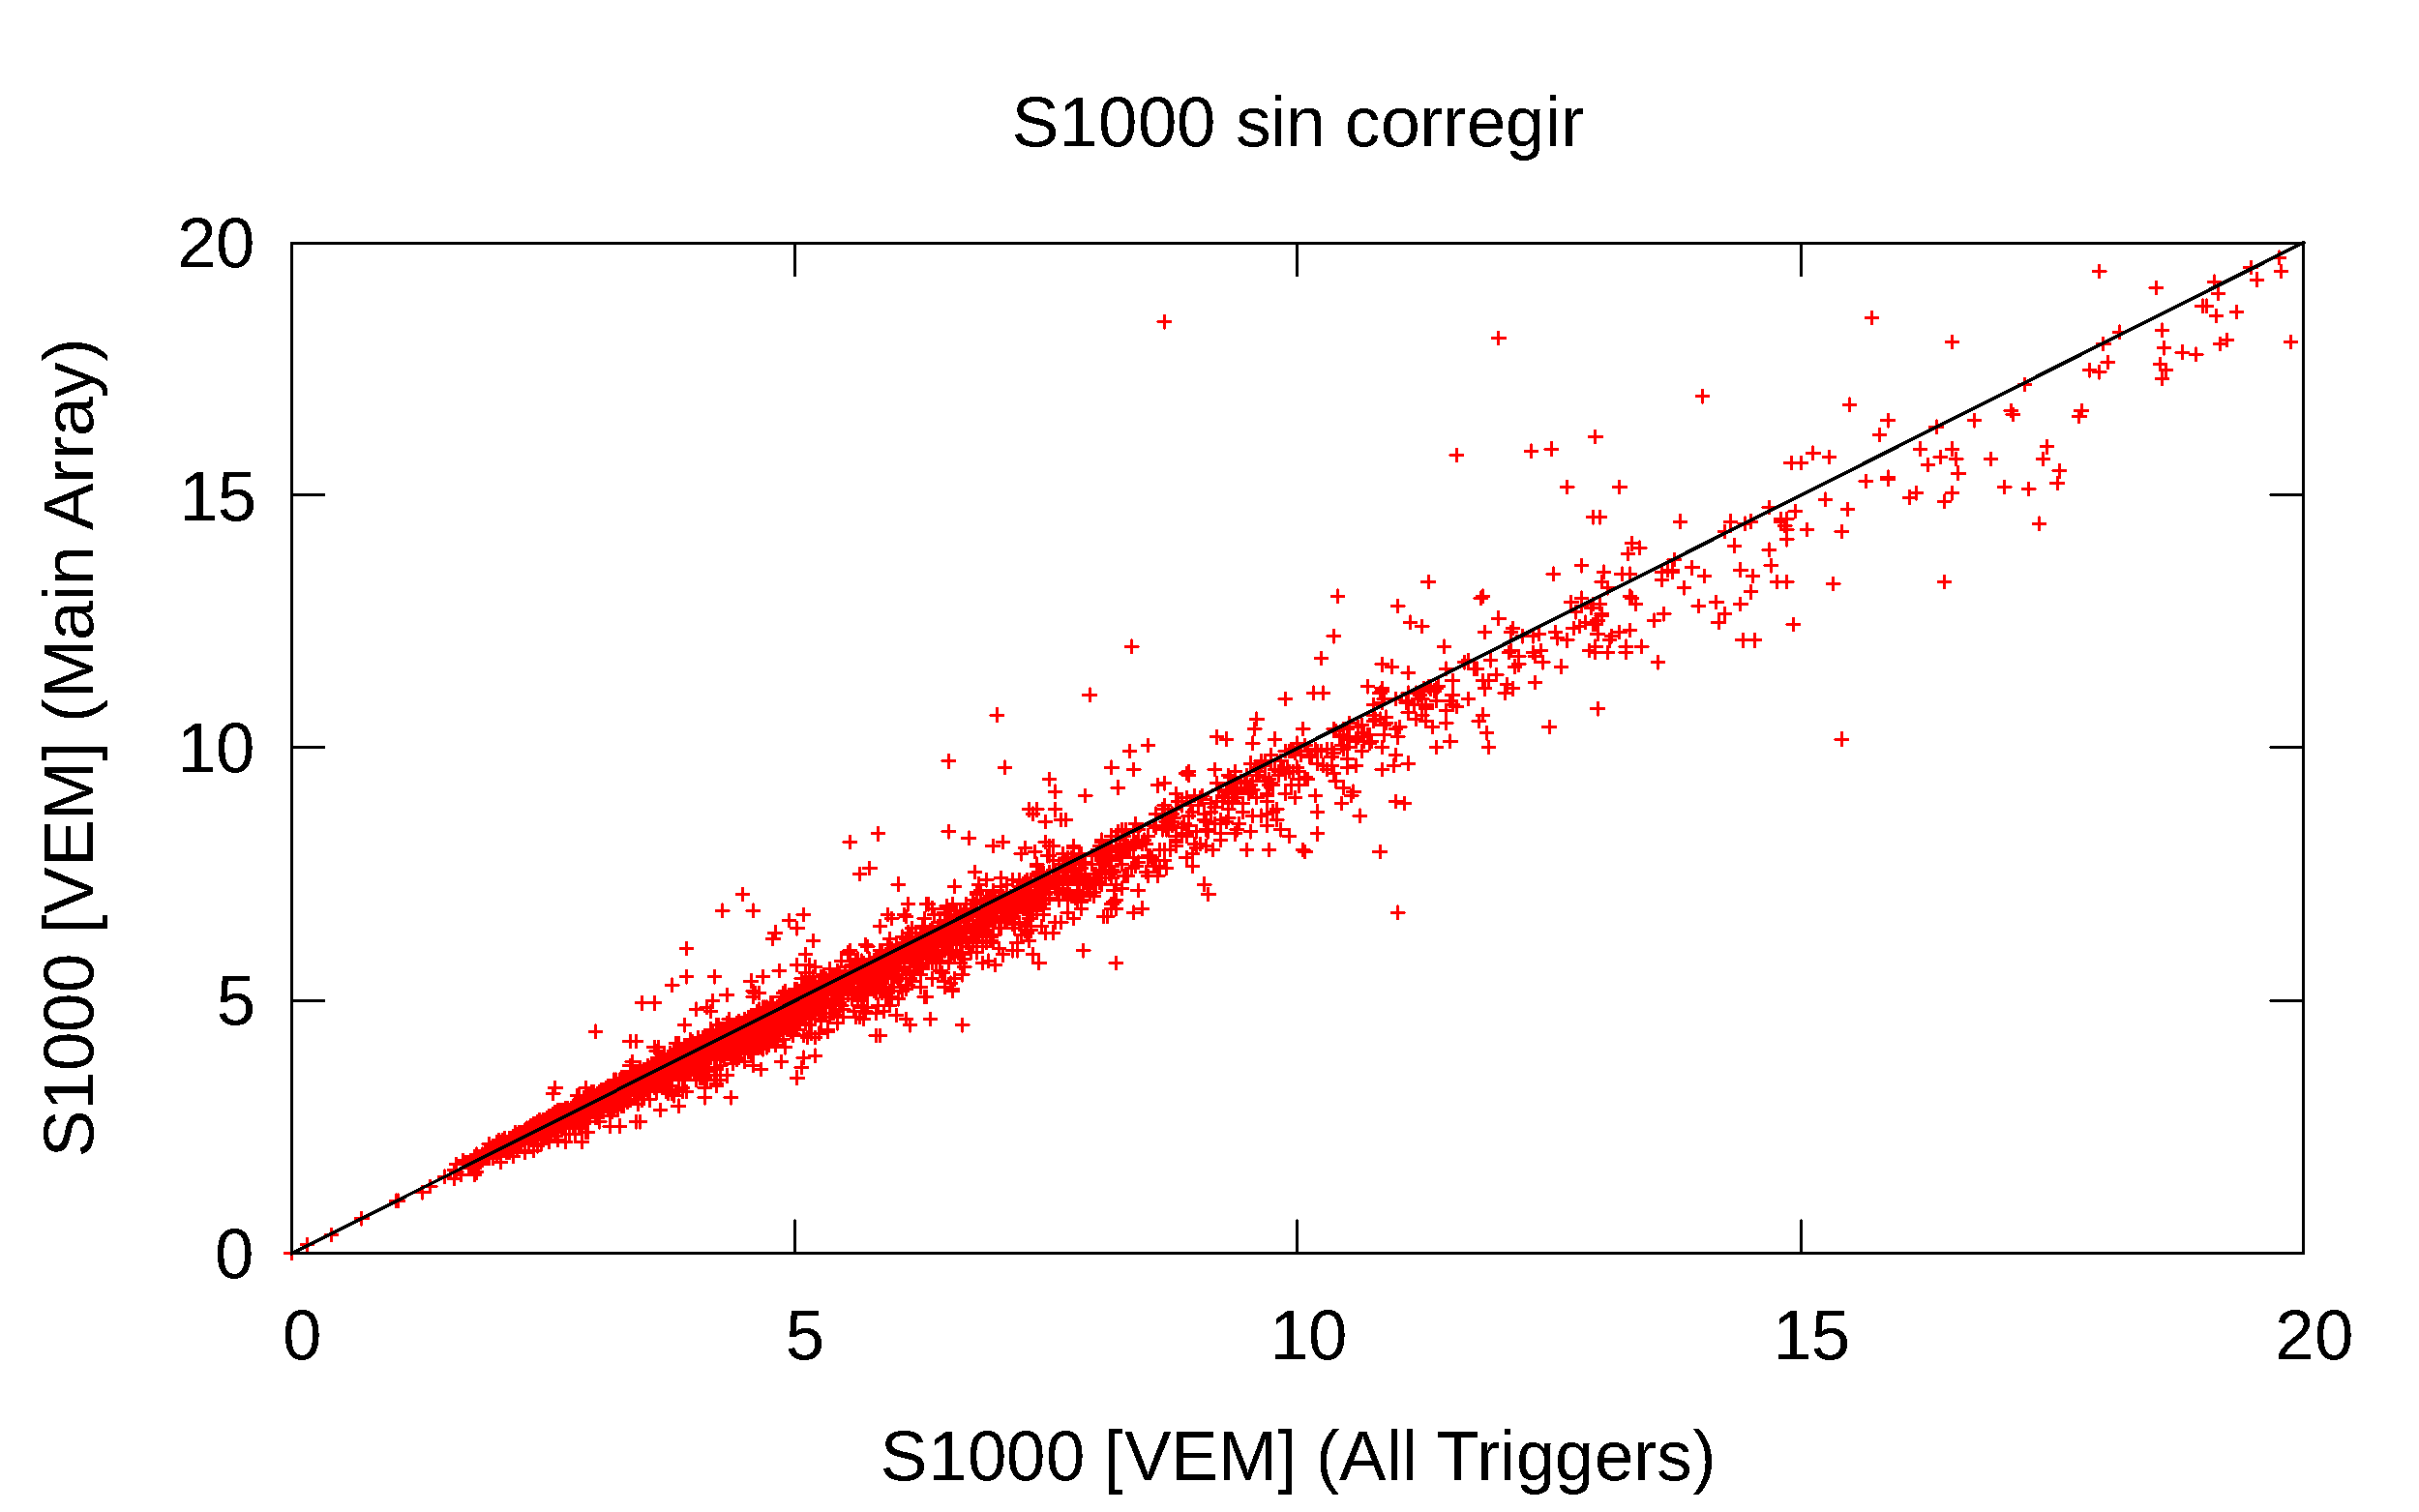
\includegraphics[width=0.5\textwidth]{s1000_versus_v2.pdf}
        \end{center}
        \caption{Valor de S1000 sin corregir por el clima según los disparos utilizados }
        \label{fig:s1000versus}
    \end{small}
\end{figure}


La Fig.\,\ref{fig:s38versus} se muestra el valor de S38, ya corregido por el clima, se observa que la señal s38 para un evento de AT tiene a ser mayor que los observado con el MA.

\begin{figure}[H]
    \begin{small}
        \begin{center}
            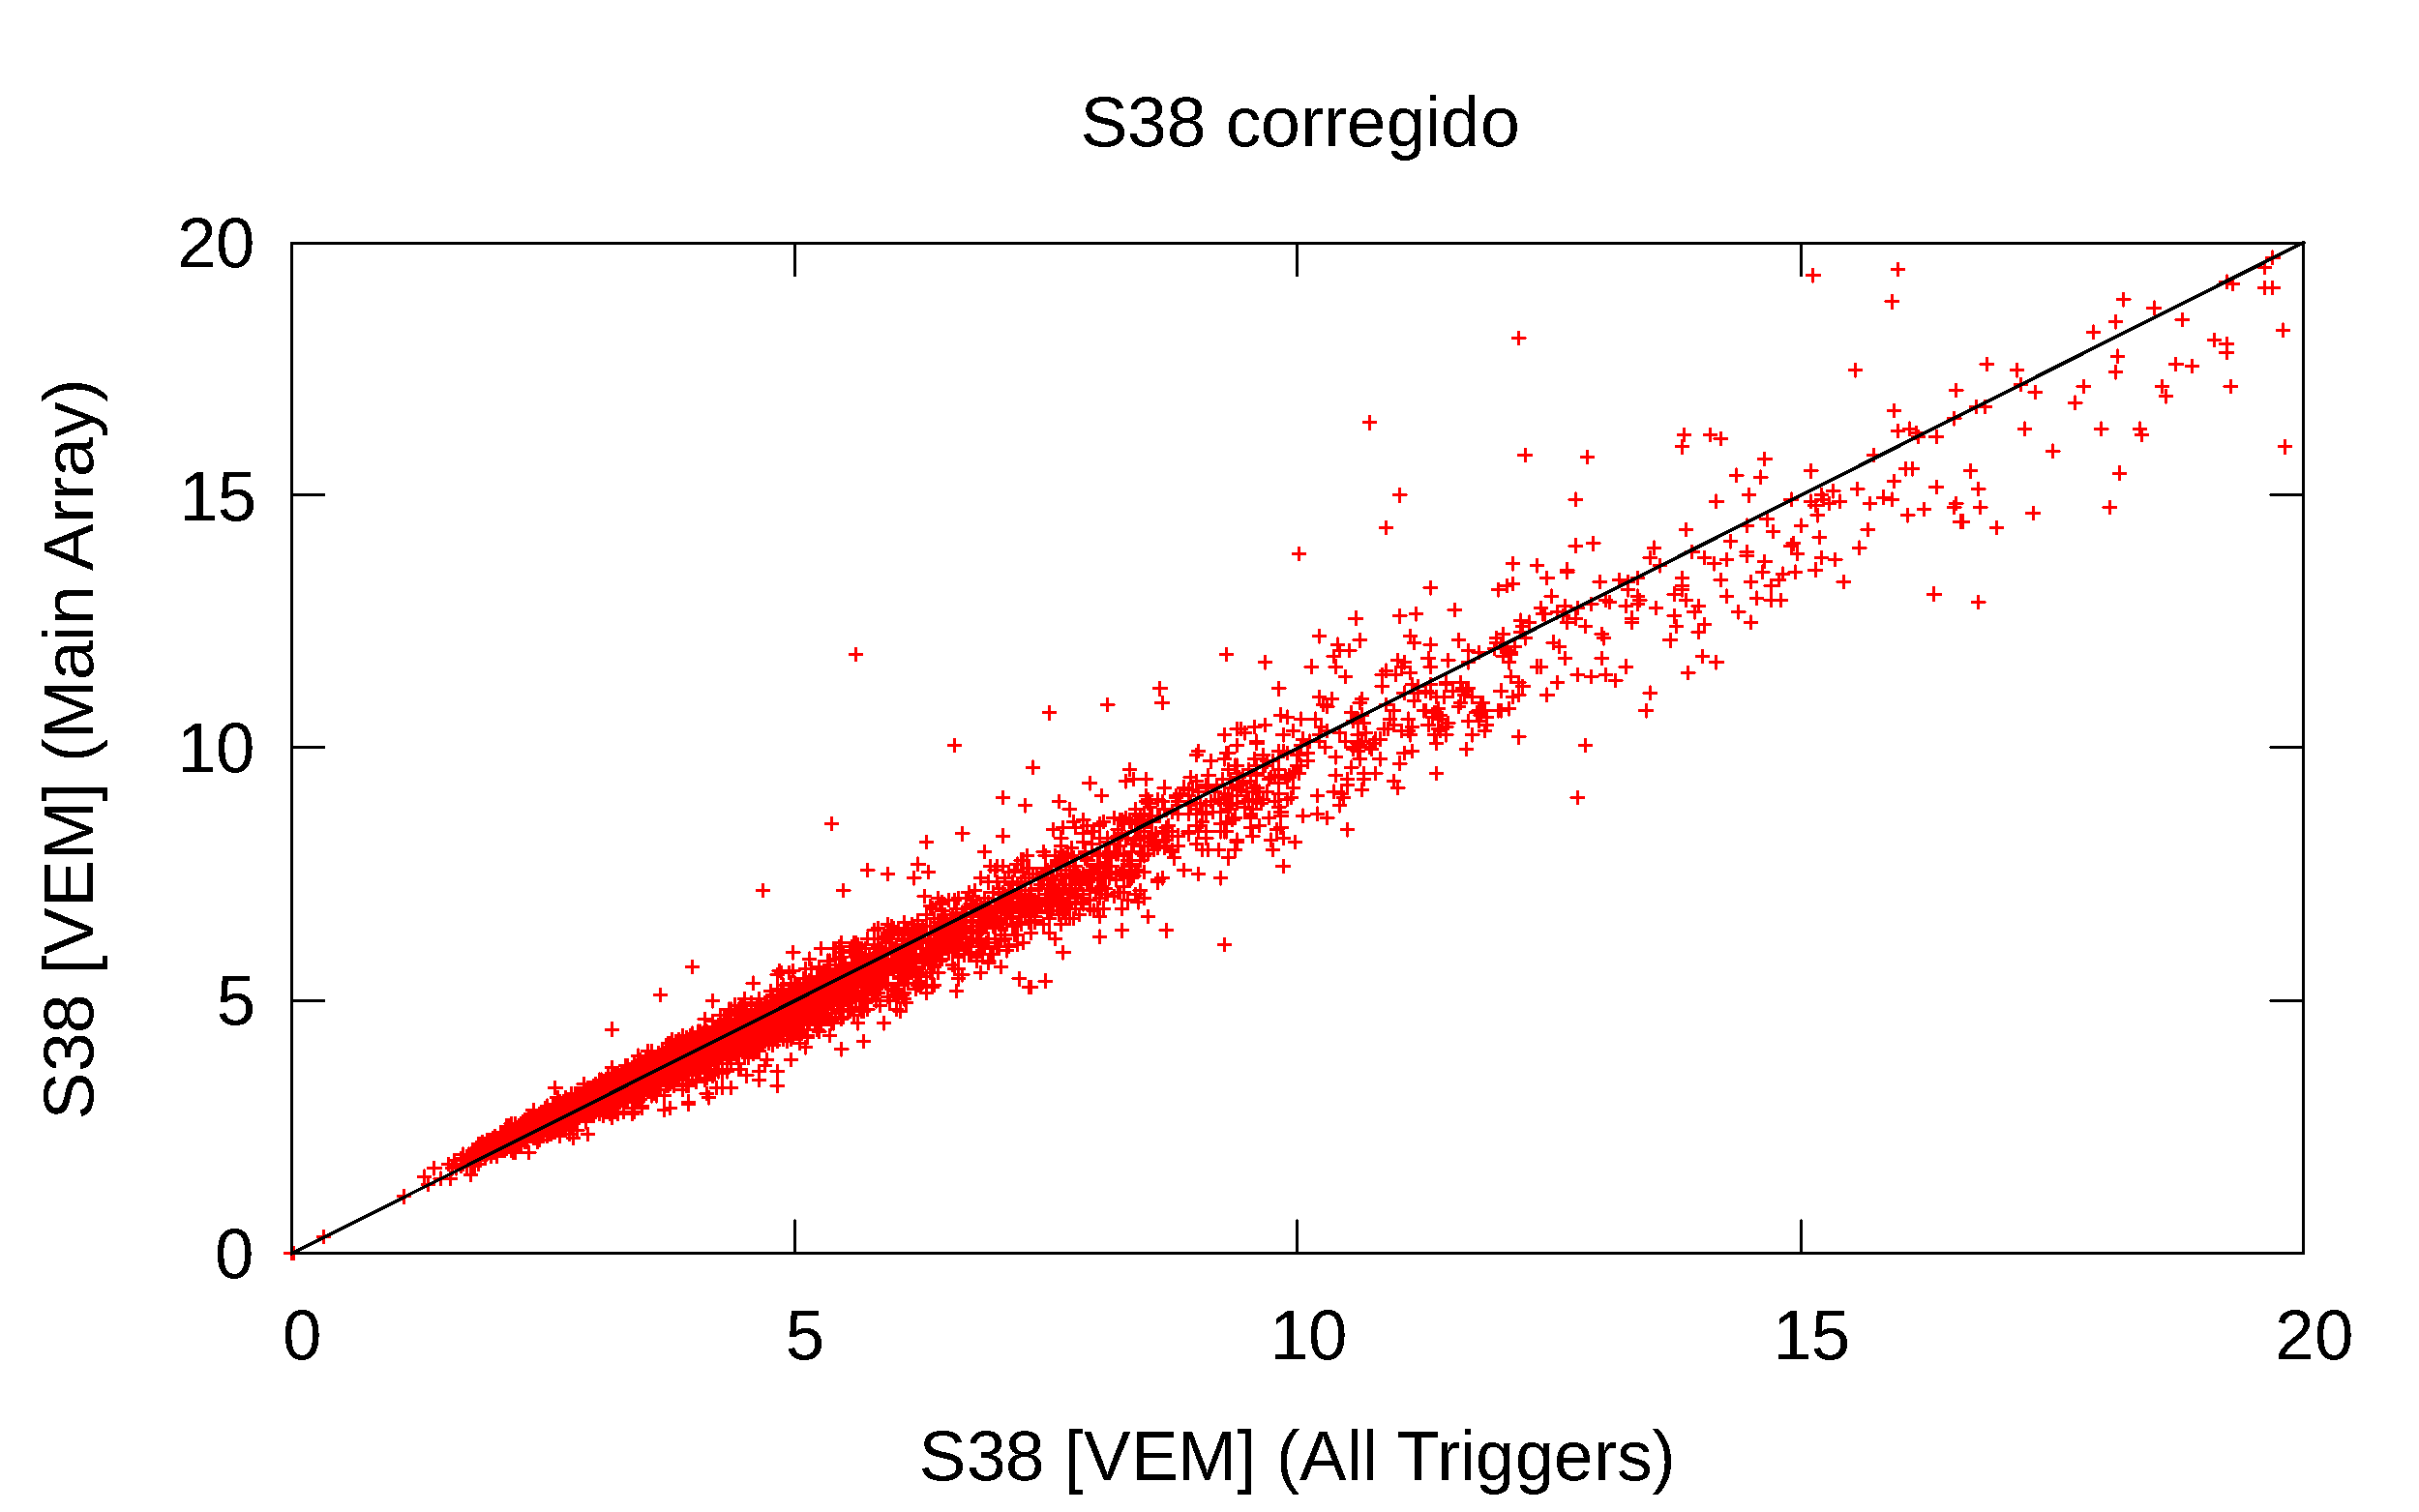
\includegraphics[width=0.5\textwidth]{s38_corregido_versus_v2.pdf}
        \end{center}
        \caption{Valor de S138 corregido por el clima según los disparos utilizados. }
        \label{fig:s38versus}
    \end{small}
\end{figure}


En la figura \ref{fig:energiaversus} de  la energía se ve como la tendencia es a que la energía de All Triggers tiende a ser mayor la energía del MA, ya que los puntos se sitúan por debajo de la línea negra.

\begin{figure}[H]
    \begin{small}
        \begin{center}
            \includegraphics[width=0.5\textwidth]{energía_corregida_versus_v2.pdf}
        \end{center}
        \caption{Valor de energía corregida según el triggers }
        \label{fig:energiaversus}
    \end{small}
\end{figure}


\section*{Acerca de la distribución de eventos por $\sin^2\theta$}

En la Fig.\ref{fig:distri} se muestran las distribuciones  para el MA y AT durante los años 2014-2020 y para el MA  entre el 2004-2014. Los eventos considerados son por encima de $3\,$ EeV, donde el MA tiene Full-efficiency.  En el rango 2004-2014 en el MA, no se observa la tendencia creciente con $\sin^2\theta$ como con las otras curvas.

\begin{figure}[H]
    \begin{small}
        \begin{center}
            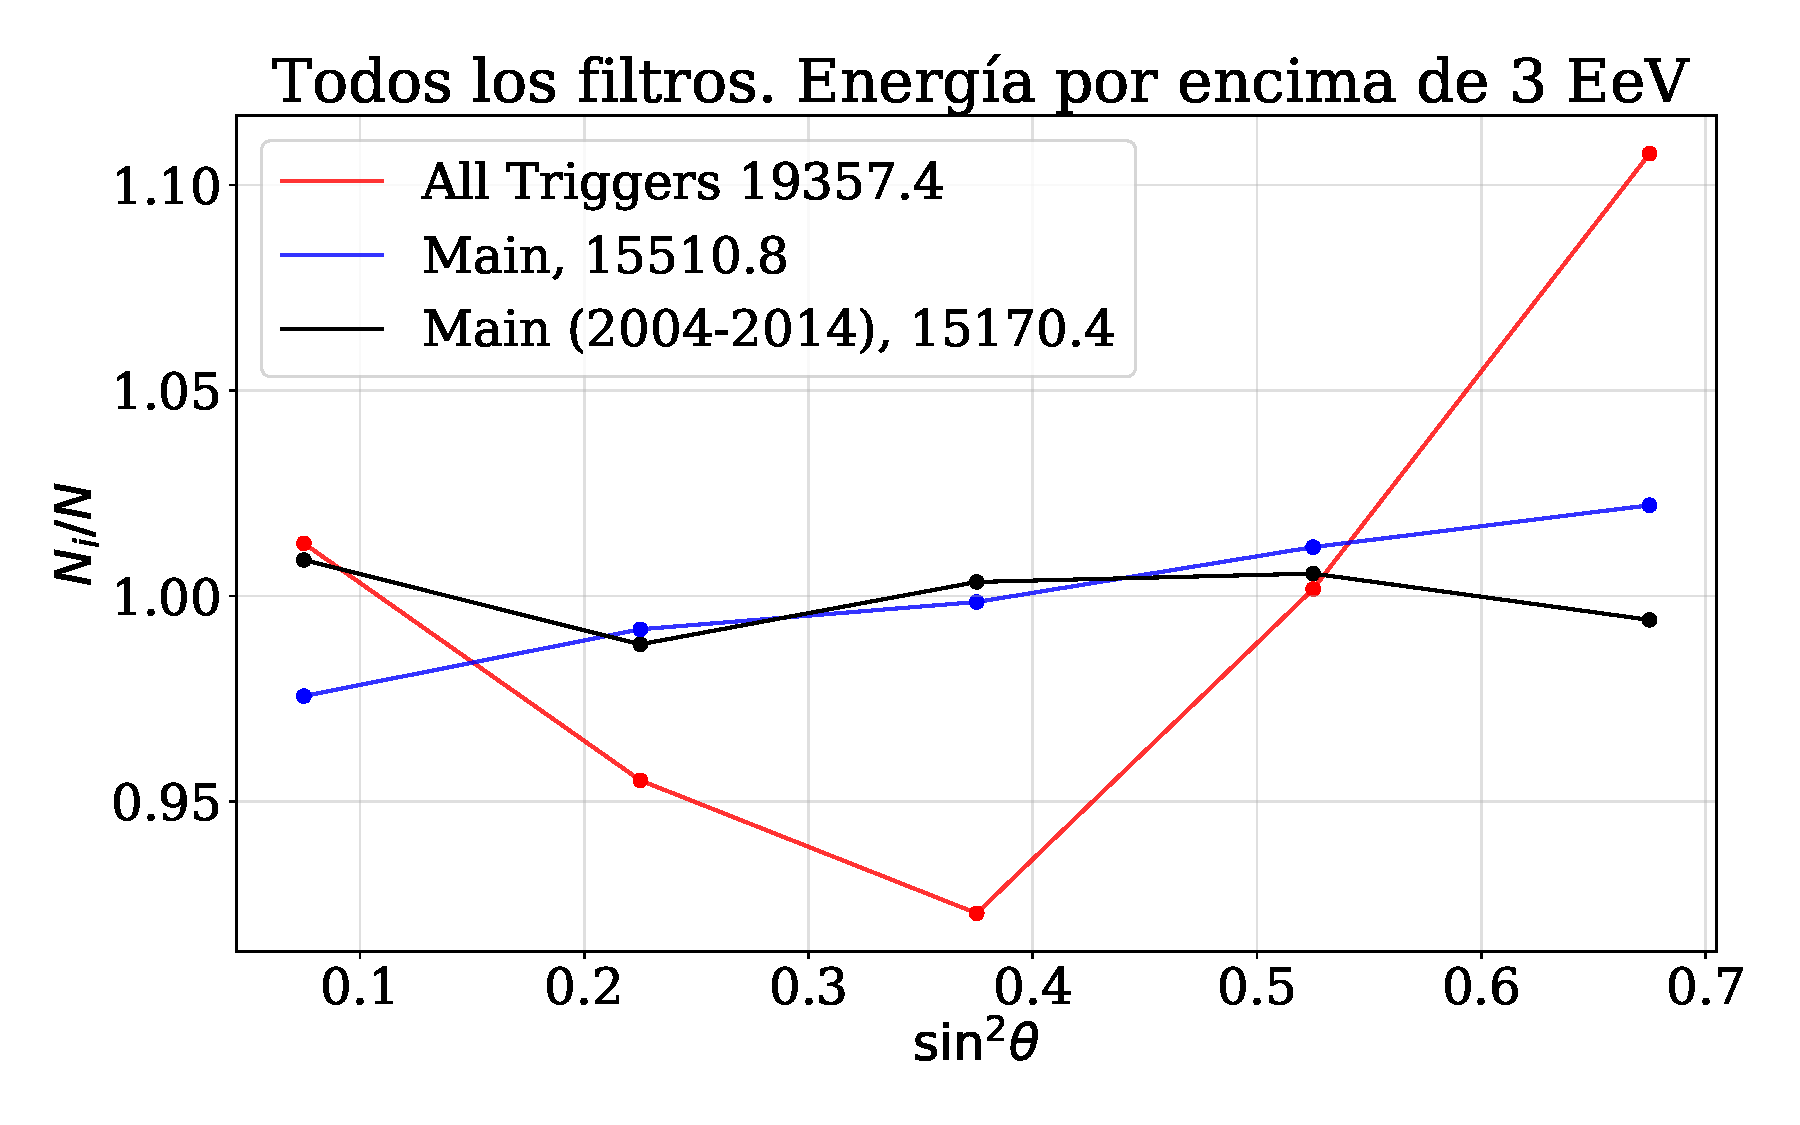
\includegraphics[width=0.5\textwidth]{eventos_bin_sin_theta.pdf}
        \end{center}
        \caption{Distribución de eventos por $\sin^2\theta$ para distintos periodos. }
        \label{fig:distri}
    \end{small}
\end{figure}

\section*{(Incompleto) Los parámetros del clima y la anisotropía mediante Rayleigh}

Existen dos archivos: \verb|ArchivoEnergia|  y \verb|ArchivoS38|, ambos con datos del conjunto de datos All Triggers.

\begin{itemize}
    \item \verb|ArchivoEnergia|: son los eventos filtrados según la energía como está en el archivo del Herald. El trabajo está centrado en el rango 1-2 EeV. El mismo  tiene $1\,081\,846$ eventos entre el 2014-2020. 
    
    \item \verb|ArchivoS38|: son archivos filtrados mediante el valor de S38 sin corregir por el clima. En la licenciatura, se tomó un valor de $5.36$ VEM como referencia a un valor de señal sin corrección del clima,  correspondiente a un evento de 1 EeV. Eso no se modificó para All Triggers. Usando los valor de A y B, se pueden obtener el valor de señal para 2 EeV que es $\sim 10.25$ VEM. Este archivo  tiene $1\,206\,582$ eventos entre el 2014-2020.
    
    \begin{itemize}
        \item Señal S38 sin corregir: Los archivos del Herald tienen dos columnas de S1000: corregida por weather y sin corregir. La columna de S38 se verificó que está corregida por el clima. Por lo que para obtener el S38 sin corregir se calcula $S38_{raw} =S38_W *(S1000_{raw}/S1000_W) $
    \end{itemize}
\end{itemize}






\end{document}